\documentclass[conference]{IEEEtran}

\IEEEoverridecommandlockouts %To add sponsors and index terms

\usepackage{cite}

\ifCLASSINFOpdf
   \usepackage[pdftex]{graphicx}
  % declare the path(s) where your graphic files are
   \graphicspath{{../images/}}
  % and their extensions so you won't have to specify these with
  % every instance of \includegraphics
   \DeclareGraphicsExtensions{.pdf,.jpeg,.png}
\else
\fi

\usepackage[cmex10]{amsmath}
\usepackage[hidelinks]{hyperref}
%for columns spanning multiple rows in tables
\usepackage{multirow}
%use the booktabs package to get (much!) better vertical spacing above and below "rules" (horizontal lines), resulting in a much more professional look of your tables.
%use the colortbl package to add color to tables.
\usepackage{booktabs,colortbl}

\usepackage{amsfonts}

% correct bad hyphenation here
\hyphenation{op-tical net-works semi-conduc-tor}

  \renewcommand\footnoterule{\vspace*{-3pt}%
     \hrule width 2in height 0.4pt
     \vspace*{2.6pt}}

\begin{document}
%
% paper title
% can use linebreaks \\ within to get better formatting as desired
\title{Temperature-based Instanton Analysis: \\
Identifying Vulnerability in Transmission Networks}


% author names and affiliations
% use a multiple column layout for up to two different
% affiliations
\author{%

\IEEEauthorblockN{Jonas Kersulis,\\ Ian Hiskens}
%\IEEEauthorblockA{Electrical Engineering and Computer Science\\
\IEEEauthorblockA{Elec. Eng. and Computer Science \\
University of Michigan\\
Ann Arbor, MI, United States\\}
\and
\IEEEauthorblockN{Michael Chertkov,\\Scott Backhaus}
%\IEEEauthorblockA{Center for Nonlinear Studies\\
\IEEEauthorblockA{Center for Nonlinear Studies\\
Los Alamos National Laboratory\\
Los Alamos, NM, United States\\
}
\and
\IEEEauthorblockN{Daniel Bienstock\\ \hspace{1pt} }
%\IEEEauthorblockA{Industrial Engineering and Operations Research\\
\IEEEauthorblockA{Ind. Eng. and Operations Research\\
Columbia University\\
New York, NY, United States\\
}

% use \thanks{} to gain access to the first footnote area
% a separate \thanks must be used for each paragraph as LaTeX2e's \thanks
% was not built to handle multiple paragraphs
%

% Who are our sponsors?
%\thanks{Identify applicable sponsor/s here. \emph{(sponsors)}}%
\thanks{\emph{The authors acknowledge the support of the Los Alamos National Laboratory Grid Science Program, subcontract 270958.}}%
}

% make the title area
\maketitle

%ABSTRACT
\begin{abstract}
A time-coupled instanton method for characterizing transmission
network vulnerability to wind generation fluctuation is presented. To
extend prior instanton work to multiple-time-step analysis, line
constraints are specified in terms of temperature rather than
current. An optimization formulation has been developed that
determines the minimum deviation in wind power from the forecast such
that line temperature is driven to its limit. Results are shown for an
IEEE RTS-96 system with several wind farms.
\end{abstract}

%INDEX TERMS
% The author shall provide up to 4 keywords (in alphabetical order) to help identify the major topics of the paper. The thesaurus of IEEE indexing keywords is posted at http://www.ieee.org/organizations/pubs/ani_prod/keywrd98.txt
\begin{IEEEkeywords}
Forecast uncertainty, Optimization, Transmission operations, Wind energy
\end{IEEEkeywords}


\section{Introduction}

The prevalence of renewables in modern transmission networks has researchers and system operators asking: What happens when the wind changes, and could fluctuations harm the grid? The instanton problem provides an answer, and this paper extends instanton analysis to the temporal setting. Though small deviations from wind forecasts are typically harmless, it is possible for certain wind generation patterns to drive the system to an infeasible operating point. Out of all troublesome wind generation patterns, the one that deviates least from the forecast is called the instanton. Instanton analysis uses optimization to find the set of troublesome wind patterns (each of which is guaranteed to cause a particular line to encounter its current flow limit). By ranking these wind patterns according to distance from forecast, we can characterize the system's vulnerability to forecast inaccuracy and enable system operators to prepare in advance.

Previous work has solved several variants of the instanton problem. In 2012 \cite{baghsorkhi2012} used the physically accurate AC power flow equations and found instanton candidates with an iterative scheme. Other papers, including \cite{chertkov2011} and \cite{chertkov2011a}, have used the DC power flow approximation to turn instanton analysis into a convex problem with an analytic solution. Current instanton research is exploring the trade-off between problem complexity and solution accuracy, with the goal of developing the most accurate model that remains convex (and therefore guarantees a solution). To the authors' knowledge, all instanton work to date has focused on instantaneous vulnerability. In other words, prior work has assumed fixed demand and generator dispatch, and has used power or current limits as constraints. Thus, the troublesome wind patterns uncovered by instanton analysis may be fleeting.

It is safe to temporarily operate a line above its current limit. Transmission system operators know this and periodically allow lines to operate above their limits to promote smooth operation under heavy load (see the introduction of \cite{banakar2005} for a history of dynamic line rating starting in the 1970s). It takes time for a line to accumulate enough heat to cause it to sag to an unacceptable level (as defined by statute and nearby tree limbs). As long as the line is allowed to cool before reaching this point, no harm will be done. If an operator is comfortable with temporarily overloaded lines, information from today's instanton analysis may be too conservative to aid in decision making.

In this paper we bring instanton analysis into the temporal setting. We consider multiple time steps and replace line current limits with heat constraints. A line's temperature change is a function of heat input (primarily Ohmic losses and heat from the sun) and dissipation (convection and radiation, which depend on ambient conditions), and is represented as a differential equation (see Section 3.4 of \cite{ieee2007} for a standard set of equations governing line temperature dynamics). Ohmic loss heating is proportional to the square of current, and dissipation is related primarily to ambient temperature and wind speed. By modeling line temperature over a significant time horizon, the new method discovers multiple-time-step wind patterns that are both likely to occur and sure to induce excessive sagging for at least one line in the network.

%generate two instanton candidates for each line in the network (one for each flow direction) using the aforementioned optimization approach.

%Instanton analysis may also be viewed as an optimal control problem. The goal is to drive the system to the edge of its feasible operating region while minimizing the ``effort'' of wind variation. We want to find the smallest deviation from a wind forecast that will drive enough current through at least one line to send it to its thermal limit. It is easy to check whether a particular wind forecast will lead to a line exceeding its thermal threshold; instanton analysis provides us with the sensitivity of line overloads to changes in the given forecast.

%If the relationship between generation and heat input was linear, we would have a linear optimal control problem.

\section{Problem formulation}

Though most of the modeling and detail of previous instanton work carries over to time-coupled analysis, there is one significant complication:  the nonlinearity of Ohmic heating (power loss) on a line. Heat input into a line is proportional to the square of the line's current. Thus, heat-constrained, time-coupled instanton analysis is a quadratically-constrained quadratic program (QCQP). QCQPs are NP-hard in general; reasonable solutions may exist, but unless the quadratic constraint matrices are positive-definite there is no solution guarantee (see \cite{mehanna2014}). Because system operators must be able to reliably obtain reasonable output from the analysis, ``no solution found'' is an unacceptable output. With this criterion in mind, we proceed to develop models for line losses, line temperature, and instanton optimization that keep integer variables to a minimum.
%We then relax this constraint to avoid introducing integer variables into the formulation, as described in \cite{almassalkhi2014}. The resulting optimization problem is convex and easily solved.

%The equations governing AC power flow are nonlinear. If we use these equations to balance the power flows in our optimization, the resulting feasible region will be nonconvex. Previous instanton work has addressed this issue by replacing the AC power flow equations with DC equations (the DC power flow equations assume that the network is lossless, with all voltage magnitudes equal to 1 per unit). This substitution renders the feasible region of instanton optimization (in the absence of nonlinear constraints) convex. 

%There are two primary difficulties associated with time-coupled instanton analysis. First, every active and reactive power flow is related to all variables involved in the flow:  the voltage magnitudes at both nodes and the angle difference between them. If we allow this tight coupling into our optimization framework, there will be no guarantee of a unique solution, or indeed of any solution at all. The second difficulty arises from the equation for power loss. Power loss on a line is proportional to the square of the current through it. This nonlinear relationship leads to nonconvexity in the optimization problem's feasible region. In this paper we address the first concern by using the DC power flow, and we sidestep the second difficulty by using a piecewise-continuous convex relaxation of the power loss equation.

\subsection{Line losses}
Starting with the AC line loss expression, \cite{almassalkhi2014} derived the following approximate relationship between line losses and voltage angle differences:
\begin{align}
\label{LL:activeLoss}
f_{ij}^{\text{loss}} &\approx r_{ij}\left(\frac{\theta_{ij}}{x_{ij}}\right)^2
\end{align}
where $f_{ij}$ is the active power flow from node $i$ to node $j$. This expression is predicated on three assumptions: voltage magnitudes are all 1 pu, cosine may be approximated by its second-order Taylor expansion, and $x_{ij} \geq 4r_{ij}$ (line reactance is at least four times as great as resistance). Equation \eqref{LL:activeLoss} simplifies the full AC line loss formulation using DC assumptions, but remains nonlinear.

%The piecewise-linear approximation described in \cite{almassalkhi2014} enables us to write a meaningful line loss constraint as a set of $S$ linear constraints, each with width $\Delta \theta$. The slope of a line $s$ from this set is
%\begin{align}
%\label{LL:segments}
%\alpha_{ij}(s) &= (2s-1)\frac{r_{ij}}{x_{ij}^2}\Delta\theta~.
%\end{align}
%Now we define new variables
%$\theta_{ij}^{\text{PW}}(s)\in[0,~\Delta\theta], \forall s \in \{1,\ldots,S\}$ so that
%\begin{align}
%\lvert \theta_{ij}\rvert &= \sum_{s=1}^S \theta_{ij}^\text{PW}(s)~,
%\end{align}
%and we can approximate line losses by
%\begin{align}
%f_{ij}^{\text{loss}} \approx \text{PWL}\left\lbrack \frac{r_{ij}}{x_{ij}^2}\lvert\theta_{ij}\rvert^2 \right\rbrack = \sum_{s=1}^S \alpha_{ij}(s) \theta_{ij}^\text{PW}(s)~.
%\end{align}
%Note that PWL$(\cdot)$ denotes the piecewise-linear approximation. There is one term for each line segment. Each term's magnitude is determined by two parameters: the segment's slope, $\alpha_{ij}(s)$, and how far along the segment we must go (with the maximum for each segment being $\Delta\theta$). Implementation of this PWL loss formulation requires integer variables to ensure that when a certain segment $s$ has $\theta_{ij}^\text{PW}(s)> 0$, every segment to its left has $\theta_{ij}^\text{PW}$ at the maximum value $\Delta\theta$. 

%%In \cite{almassalkhi2014} it was shown that if we relax this adjacency condition, we obtain an integer-free bounded convex relaxation of PWL$(\cdot)$:
%%\begin{align}
%%\text{PWL}\left\lbrack \frac{r_{ij}}{x_{ij}^2}\lvert\theta_{ij}\rvert^2\right\rbrack &\leq \sum_{s=1}^S \alpha_{ij}(s)\theta_{ij}^\text{PW}(s)\equiv f_{ij}^\text{loss}
%%\end{align}
%%This relaxed line loss formulation can overestimate losses. 

%The only remaining issue pertains to the absolute value constraint in the definition of the $\theta_{ij}^\text{PW}$ variables. We can represent each angle difference as the sum of two components:
%\begin{align}
%\theta_{ij} &= \theta_{ij}^+ - \theta_{ij}^-\\
%\implies \sum_{s=1}^S \theta_{ij}^\text{PW} &= \theta_{ij}^+ + \theta_{ij}^-
%\end{align}
%This formulation is only tight when one of the two components is zero. Complementarity is enforced with integer variables.
%%but \cite{almassalkhi2014} shows this is not necessary so long as 1) losses are fixed in the power balance equations, and 2) the objective function penalizes temperature changes.
%The previous discussion may be summarized by the set of equations:
%\begin{subequations}
%\label{LL:floss}
%\begin{align}
%f_{ij}^\text{loss} &= \frac{r_{ij}}{x_{ij}^2}\Delta\theta \sum_{s=1}^S (2s-1)\theta_{ij}^\text{PW}(s)\\
%\sum_{s=1}^S \theta_{ij}^\text{PW}(s) &= \theta_{ij}^+ + \theta_{ij}^-\\
%\theta_{ij} &= \theta_{ij}^+ - \theta_{ij}^-\\
%\theta_{ij} &\in(-\theta_{max},\theta_{max})\\
%\theta_{ij}^+,\theta_{ij}^- &\geq 0\\
%\theta_{ij}^\text{PW}(s) &\in [0,\Delta\theta]
%\end{align}
%\end{subequations}

\subsection{Line temperature dynamics}
According to analysis done in \cite{almassalkhi2014} (which is based on \cite{ieee2007}), changes in line temperature may be calculated using the following Euler integration:
\begin{align}
\label{TD:euler}
\Delta T_{ij}[t+1] &= \tau_{ij}\Delta T_{ij}[t] + \rho_{ij}\Delta f_{ij}^\text{loss}[t] + \delta_{ij}\Delta d_{ij}[t]~,
\end{align}
where the initial condition is $\Delta T_{ij}[0] = 0$. $\tau_{ij}$ and $\bar{\gamma}_c$ are defined as
\begin{align}
\tau_{ij} &= 1 - \frac{T_s\bar{\gamma}_c}{mC_p},& \bar{\gamma}_c &= \eta_c + 4\eta_r(T^\text{lim} + 273)^3~,
\end{align}
and $\rho_{ij} = T_s/mC_p$. Finally, $\Delta d_{ij} = \text{col}(\Delta q_{s,ij},\Delta T_\text{amb})$, and $\delta_{ij}$ represents exogenous inputs and is equal to $[\rho_{ij}~\gamma_{ij}]$, where
\begin{align}
\gamma_{ij} &= \frac{T_s\bar{\gamma}_a}{mC_p}, & \bar{\gamma}_a &= \eta_c + 4\eta_r(T_\text{amb}^* + 273)^3~.
\end{align}
The parameters in this line temperature model are described in Table \ref{tab:heatparams}.

\newcommand{\splitcell}[2][c]{%
  \begin{tabular}[#1]{@{}c@{}}#2\end{tabular}}
  
\begin{table}
\begin{center}
\caption{Line heating parameters}
\label{tab:heatparams}
\begin{tabular}{|c|c|c|}
	\hline
	         Parameter           &   Units    &               Description                \\ \hline
	           $T_s$             &    $s$     &               Sample time                \\ \hline
	           $mC_p$            & $J/(m\cdot C)$ & \splitcell{Per-unit-length heat capacity\\of the conductor}         \\ \hline
	          $\eta_c$           & $W/(m\cdot C)$ &     \splitcell{Conductive heat loss \\ rate coefficient}         \\ \hline
	          $\eta_r$           & $W/(m\cdot C)$ &      \splitcell{Radiative heat loss\\rate coefficient}         \\ \hline
	       $T^\text{lim}$        &    $C$     &      \splitcell{Line temperature at\\steady-state current limit.}   \\ \hline
	       $\Delta q_{s,ij}$ & $W/m$ & \splitcell{Solar heat input\\ into conductor} \\ \hline
	       $\Delta T_\text{amb}$ & C & \splitcell{Change in \\ambient temperature} \\ \hline
\end{tabular} 
\end{center}
\end{table}

For numerical stability, we need $\tau_{ij}\in(-1,1)$, which leads to the following constraint on sampling time for the integration:
\begin{align}
\label{TD:sample}
T_s < \min_{ij}\left\lbrace \frac{2mC_{p,ij}}{\bar{\gamma}_{c,ij}}\right\rbrace
\end{align}

Having introduced the necessary equations for modeling line temperature, we now recognize \eqref{TD:euler} as a relationship between angle differences and constants. Note that \eqref{TD:euler} is a recursive relationship between temperature at time $t+1$ and temperature at time $t$. Repeatedly substituting into this equation and using \eqref{LL:activeLoss}, we find the following expression for change in line temperature at time $t^*$:
%
%\begin{align*}
%\Delta T_{ij}[t+1] &= \tau_{ij}\Delta T_{ij}[t] + \rho_{ij}\Delta f_{ij}^\text{loss}[t] + \delta_{ij}\Delta d_{ij}[t]\\
%&= \tau_{ij}\left\lbrace \tau_{ij} \Delta T_{ij}[t-1] + \rho_{ij}\Delta f_{ij}^\text{loss}[t-1] + \delta_{ij}\Delta d_{ij}[t-1] \right\rbrace + \rho_{ij}\Delta f_{ij}^\text{loss}[t] + \delta_{ij}\Delta d_{ij}[t]\\
%\end{align*}

\begin{align}
\label{TD:condensed}
\Delta T_{ik}[t^*] &= \frac{\rho_{ik} r_{ik}}{x_{ik}^2}\sum_{t=1}^{t^*}\tau_{ik}^{t-1}\theta_{ik}^2[t^*-t]~ + \\
\nonumber &\quad + \delta_{ik} \sum_{t=1}^{t^*}\tau_{ik}^{t-1}\Delta d_{ik} [t^* - t]
\end{align}
The first term in Equation \eqref{TD:condensed} varies with angle differences. The second term, which is based on external conditions, is constant with respect to all power flow variables. Moving all constants to the left-hand side, we find:
%We can, therefore, re-write the constraint \eqref{I:lim} as
%\begin{align}
%\label{TD:new}
%\Delta T_{ik}[t^*] - \delta_{ik} \sum_{t=1}^{t^*}\tau_{ik}^{t-1}\Delta d_{ik} [t^* - t]  &= \\
%\nonumber = \frac{\rho_{ik}r_{ik}}{x_{ik}^2} \sum_{t=1}^{t^*} \tau_{ik}^{t-1}\theta_{ik}^2[t^* - t]
%\end{align}

\begin{multline}
\label{TD:new}
\Delta T_{ik}[t^*] - \delta_{ik} \sum_{t=1}^{t^*}\tau_{ik}^{t-1}\Delta d_{ik} [t^* - t]  = \\
 = \frac{\rho_{ik}r_{ik}}{x_{ik}^2} \sum_{t=1}^{t^*} \tau_{ik}^{t-1}\theta_{ik}^2[t^* - t]
\end{multline}
The left side of \eqref{TD:new} is constant during optimization, and the right side is a weighted, scaled two-norm of the vector of angle difference variables $\theta_{ik}[t],~ t\in \{1,\ldots,t^*\}$. Now we define
\begin{align}
\boldsymbol{\theta}_{ik} &:= \begin{bmatrix}\theta_{ik}[0]^2 & \theta_{ik}[1]^2 & \cdots & \theta_{ik}[t^*-1]^2 \end{bmatrix}^\top \\
\boldsymbol{\tau}_{ik} &:= \begin{bmatrix} \tau_{ik}^{t^*-1} & \tau_{ik}^{t^*-2} & \cdots & 1 \end{bmatrix}^\top \\
\boldsymbol{\Delta d}_{ik} &:= \begin{bmatrix}
\Delta d_{ik}[0] & \Delta d_{ik}[1] & \ldots ~~ \Delta d_{ik}[t^*-1] 
\end{bmatrix}^\top
\end{align}
Note that these three vectors are implicit functions of $t^*$, but this dependence is hidden in their notation to promote conciseness. Having defined these three vectors, we can express \eqref{TD:new} as follows:
\begin{align}
\label{TD:vectors}
\Delta T_{ik}[t^*] - \delta_{ik} \boldsymbol{\tau}_{ik}^\top \boldsymbol{\Delta d}_{ik}  &= \frac{\rho_{ik}r_{ik}}{x_{ik}^2} \boldsymbol{\tau}_{ik}^\top \boldsymbol{\theta}_{ik}
\end{align}

The temperature dynamics described in this section are used in the following development of the instanton formulation itself.

\subsection{Instanton formulation}
In the preceding discussion we have shown how to calculate losses with \eqref{LL:activeLoss} and use this information to find line temperature changes with \eqref{TD:euler}-\eqref{TD:sample} and ultimately \eqref{TD:vectors}. All that remains is to describe the instanton optimization itself.

The following equations describe an optimization problem that minimizes deviation from the wind forecast while heating a certain line to an unacceptable temperature by the last time step:
\begin{subequations}\label{I:all}
\begin{align}
\label{I:obj}\min & \sum_{t=1}^{t_\text{end}} x_t^\top Q_x x_t \\
\nonumber& \text{subject to:} \\
\label{I:flow} \sum_k Y_{ik} \theta_{ik,t} & = G_{i,t} + \rho_{i,t} + x_{i,t} - D_{i,t} ~ \forall i \in \mathcal{N},~t\in 1... T \\
\label{I:conv} G_t &= G_{0,t} + k\alpha_t \quad \forall t\in 1\ldots T \\
\label{I:slack} \theta_{k,t} & = 0 \quad \forall t\in 1\ldots T \\
\label{I:lim} \Delta T_{ik}[T] &= \Delta T_{ik}^\text{lim}\quad \text{for some }(i,k)\in \mathcal{G}
\end{align}
\end{subequations}
together with \eqref{LL:activeLoss} and \eqref{TD:euler}, where:
\begin{itemize}
\itemsep1pt\parskip0pt\parsep0pt
\item $x_{i,t}$ is the difference between actual output and forecast output at wind farm $i$ and time $t$. Thus, $x$ is a vector of wind forecast deviations.
\item $Q_x$ may be set to the identity matrix or used to encode correlation between wind sites.
\item $\rho_{i,t}$ is renewable generation forecast at bus $i$ and time $t$ in per unit 
\item $Y_{ik}$ is the $(i,k)$-th element of the admittance matrix $Y$, which
  assumes resistances throughout the network are zero.
\item $\theta_{ik,t}$ is the difference between the bus $i$ phase angle and the bus $k$ phase angle at time $t$.
\item $G_{i,t}$ is the conventional active power generation at node $i$ and time $t$.
\item $D_{i,t}$ is the active power demand at bus $i$ and time $t$.
\item $\mathcal{N}$ is the set of buses (nodes).
\item $G_t$ is the vector of conventional active power generation at time $t$.
\item $G_{0,t}$ is the scheduled conventional active power generation (without droop response).
\item $k$ is the vector of participation factors for conventional
  generators, with
\begin{equation}
\label{I:part} \sum_i k_i = 1.
\end{equation}
The case where $k_i=1$ corresponds to generator $i$ taking up all
  slack.
\item $\alpha_t$ is the participation coefficient (mismatch) at time $t$, defined as
\end{itemize}

\[\alpha_t:= \sum D_t - \sum \rho_t - \sum G_{0,t} ~.\]

\begin{itemize}
\itemsep1pt\parskip0pt\parsep0pt
\item $\Delta T_{ik}^{lim}$ is the change in temperature that will push line $(i,k)$ to its thermal limit.
\item $\theta_\text{ref}$ is the phase angle of the reference bus (fixed at zero).
\item $\mathcal{G}$ is the set of edges (lines).
\end{itemize}


%Consider \eqref{I:lim}. We can use \eqref{LL:activeLoss} and \eqref{TD:euler} to express this constraint in terms of squared angle difference variables:
%\begin{align*}
%\Delta T_{ik}[t_\text{end}] &= \Delta T_{ik}^\text{lim}\\
%&=  \\
% &= \tau_{ij}\Delta T_{ij}[t_\text{end}-1] + \rho_{ij}\Delta f_{ij}^\text{loss}[t_\text{end}-1] + \delta_{ij}\Delta d_{ij}[t_\text{end}-1]
%\end{align*}


Equation \eqref{I:obj} expresses the desire to find wind patterns that remain close to the wind forecast. The first constraint equation \eqref{I:flow} enforces DC power balance. The next constraint \eqref{I:conv} models conventional active power generation as a sum of
scheduled generation and droop response (where generators share the task of compensating for mismatch between total generation and total load). The system angle reference is established by \eqref{I:slack}. Last is \eqref{I:lim}, which constrains the temperature of a particular line to be equal to its limit at the final time $t_\text{end}$. By \eqref{TD:vectors}, we can express \eqref{I:lim} as
\begin{align}\label{temp}
\Delta T_{ik}[T] - \delta_{ik} \boldsymbol{\tau}_{ik}^\top \boldsymbol{\Delta d}_{ik}  &= \frac{\rho_{ik}r_{ik}}{x_{ik}^2} \boldsymbol{\tau}_{ik}^\top \boldsymbol{\theta}_{ik}~.
\end{align}
Because the slack bus is specified to be bus $k$ in \eqref{I:slack}, \eqref{I:lim} may be viewed as an equality constraint on the vector of squared angle variables $\theta_i[t]^2$, $t\in \{0,1,\ldots,t_\text{end}\}$. Thus, \eqref{I:all} has a quadratic objective function, a set of linear constraints, and a single quadratic constraint.

By solving \eqref{I:all} for each line $(i,k)\in\mathcal G$, we obtain a set of instanton candidate wind patterns, each of which will heat a particular line to its thermal limit. Of these candidates, the one that deviates least from the wind forecast (across all time steps) is the instanton wind pattern.

\section{Conversion to optimization problem}

If we arrange all variables into a single vector, \eqref{I:all} may be viewed as a quadratically-constrained quadratic program (QCQP) of the following form:

\begin{subequations}\label{opt}
\begin{align}
\label{opt:obj}  &&  \min z^\top Q_{obj} z &\\
\label{opt:lin} & s.t. & Az &= b  \\
\label{opt:quad} &&  z^\top Q_{\theta}z &= c 
\end{align}
\end{subequations}

The objective \eqref{opt:obj} is equivalent to \eqref{I:obj}, the linear equality constraints \eqref{opt:lin} represent \eqref{I:flow}-\eqref{I:slack}, and the quadratic equality constraint \eqref{opt:quad} is equivalent to \eqref{I:lim}. $z$ consists of $(n+n_r+1)t^*$ variables, where $n$ is the number of nodes, $n_r$ is the number of nodes with wind farms, and $t^*$ is the number of time steps.
\begin{itemize}
	\item $n_rt^*$ of these are deviation variables,
    \item $(n-1)t^*$ are angle variables,
    \item $t^*$ are mismatch variables (one per time step), and
    \item $t^*$ are angle difference variables $\hat{\theta}_{ik}$ representing the difference between $\theta_i$ and $\theta_k$ at each time step. These variables are used to convert the quadratic constraint into a norm constraint.
\end{itemize}

Thus, the vector $z$ consists of $t^*$ groups of $(n+n_r)$ variables stacked together (one for each time step), with a set of $t^*$ angle difference variables at the end. At a particular time step $t$, the group of variables is $\begin{bmatrix} x_t^\top & \theta_t^\top & \alpha_t \end{bmatrix}^\top$. $x_t$ represents deviations from forecast at the $n_r$ wind nodes, $\theta_t$ is the column of $n-1$ independent angle variables at time $t$, and $\alpha_t$ is the mismatch between generation and demand at time $t$. An instance of the temporal instanton problem is characterized by $Q_{obj}$, $A$, $b$, and $Q_{\theta}$. Following is a description of each part.

\subsection{Objective function and $Q_{obj}$}

The objective function depends solely on deviation variables $x$, so $Q_{obj}$ is a matrix that weights only the $x$ variables in $z$. If there are two time steps, for example, the vector of variables would be $z = \begin{bmatrix}x_t^\top & \theta_1^\top & \alpha_1 & x_2^\top & \theta_2^\top & \alpha_2 & \hat{\theta}\end{bmatrix}^\top$, and $Q_{obj}$ would be

\begin{align*}
Q_{obj} = \begin{bmatrix} Q_x & 0 & 0 & 0 & 0 & 0 \\ 0 & 0 & 0 & 0 & 0 & 0 \\ 0 & 0  & 0 & 0 & 0 & 0 \\ 0 & 0 & 0 & Q_x & 0 & 0 \\ 0 & 0 & 0 & 0 & 0 & 0 \\ 0 & 0 & 0 & 0 & 0 & 0\end{bmatrix}~,
\end{align*}
where $Q_x$ represents the correlation between wind farms (if any). In our RTS-96 analysis later on, we will assume $Q_x=I$, the identity matrix.

\subsection{Linear constraints: $A$ and $b$}

All constraints except the temperature limit may be grouped into a single linear equation $Az=b$. Setting aside the $\hat{\theta}_{ik}$ angle difference variables for the moment, the $A$ matrix has a block diagonal structure where each block consists of $(n+1)$ rows and $(n_r+n)$ columns. The first $n$ rows describe power balance and distributed slack behavior. We have the following equation for a non-slack node with a wind farm (with all variables on the left-hand side and constants on the right):

\begin{align*}
-x_{i,t} + \sum\limits_{k\neq s} Y_{ik}\theta_{k,t} - k_i\alpha_{i,t} &= G_{i,t}^0 + \rho_{i,t} - D_{i,t}~,
\end{align*}
where the slack node is node $s$. Rearranging, we see that this equation is simply power balance in disguise:
\begin{align}\label{pbal}
\sum\limits_{k\neq s} Y_{ik}\theta_{k,t}  &= (G_{i,t}^0 + k_i\alpha_t) + (\rho_{i,t} + x_{i,t}) - D_{i,t}
\end{align}
The first pair of terms on the right-hand side of \eqref{pbal} represents conventional generation with distributed slack -- generator $i$ is taking a portion $k_i$ of the mismatch $\alpha_t$. The second pair of terms is renewable generation: forecast $\rho_{i,t}$ plus deviation $x_{i,t}$. The final term is demand at node $i$ and time $t$. For a non-slack node with a wind farm, the equation is \eqref{pbal} without the renewable generation terms. For a slack node, we have \eqref{pbal} with the left-hand side equal to 0 (keeping track of distributed slack only). In addition to the $n$ rows corresponding to \eqref{pbal} at the $n$ nodes, there is one additional equation used to fix $\alpha_t$ (again, with variables on the left and constants on the right):

\begin{align*}
\sum_i x_{i,t} + \alpha_t &= \sum_i (D_{i,t} - G_{i,t}^0 - \rho_{i,t})
\end{align*}
Rearranging, we see that this simply fixes $\alpha_t$ to the difference between generation and demand at time $t$:

\begin{align}\label{mismatch}
 \alpha_t &= \sum_i \left(D_{i,t} - G_{i,t}^0 - (\rho_{i,t} + x_{i,t})\right)
\end{align}
From \eqref{mismatch} we see that $\alpha_t$ is positive when demand exceeds generation. This causes conventional generators to increase their output according to \eqref{I:conv}.

The previously described $(n+1)$ rows of $Az=b$ pertain to a single time step block. The $T$ total blocks are arranged diagonally to form $(n+1)T$ rows of $A$. There is one additional block of $A$ used to relate angle difference variables $\hat{\theta}_{ik}$ to angle variables $\theta_i$ and $\theta_k$. This block contains one row for each time step. At time $t$, we have:

\begin{align}\label{thetahat}
\hat{\theta}_{ik,t} &= \tau^{\frac{t^*-t}{2}}(\theta_{i,t} - \theta_{k,t})
\end{align}
Equivalence of this relationship to \eqref{temp} is discussed in the next subsection.

\subsection{Quadratic constraint: $Q_{\hat{\theta}}$ and $c$}

Recall that \eqref{temp} describes the temperature constraint on a chosen line $(i,k)$. The only variable component of the relationship is $\boldsymbol{\theta_{ik}}$, so we can express \eqref{temp} with a constant on the right-hand side that represents known ambient conditions and line parameters:

\begin{align}\label{temp2}
\sum_{t=1}^{t^*} \tau_{ik}^{t^*-t} (\theta_{i,t} - \theta_{k,t})^2 &=  \frac{x_{ik}^2}{\rho_{ik} r_{ik}} \left(\Delta T_{ik}^{lim} - \delta_{ik} \boldsymbol{\tau}_{ik}^\top \boldsymbol{\Delta d}_{ik}\right)
\end{align}
From the definition of $\hat{\theta}_{ik,t}$ in \eqref{thetahat}, we see that \eqref{temp2} may be expressed as:

\begin{align}
\sum_{t=1}^{t^*} \hat{\theta}_{ik,t}^2 &=  \frac{x_{ik}^2}{\rho_{ik} r_{ik}} \left(\Delta T_{ik}^{lim} - \delta_{ik} \boldsymbol{\tau}_{ik}^\top \boldsymbol{\Delta d}_{ik}\right)
\end{align}
With $\hat{\theta}_{ik}$ as the last $t^*$ elements of $z$, we see that the matrix $Q_{\theta}$ in \eqref{opt:quad} is a matrix of zeros with a $t^*$-by-$t^*$ identity matrix in the lower-right corner. In other words, our temperature constraint becomes

\begin{align*}
\lVert \hat{\theta}_{ik}\rVert^2 &= c^2~,
\end{align*}
where $$c = \frac{x_{ik}^2}{\rho_{ik} r_{ik}} \left(\Delta T_{ik}^{lim} - \delta_{ik} \boldsymbol{\tau}_{ik}^\top \boldsymbol{\Delta d}_{ik}\right)~. $$

\section{Solution}

The structure of \eqref{opt} is similar to that of the well-known trust-region subproblem. Here we describe a four-step solution method based in part on work from \cite{bienstock2014}.

\subsection{Translation}

The first step is to translate the problem by $z^*$, the point in the set $\{z:Az=b\}$ closest to the origin. One way to find $z^*$ is to perform a QR factorization of $A$ with a rank estimate based on its R factor. The translation itself is a change of variables from $z$ to $\bar{z}=z - z^*$. This results in the following problem:

\begin{subequations}\label{opt2}
\begin{align}
\label{opt2:obj} && \min \bar{z}^\top Q_{obj}\bar{z} + 2\bar{z}^\top Q_{obj}z^* &\\
\label{opt2:lin} & s.t. & A\bar{z} &= 0 \\
\label{opt2:quad} && \bar{z}^\top Q_{\theta}\bar{z} + z^{*\top}Q_\theta z^* - c &= 0 
\end{align}
\end{subequations}
Because of how $z^*$ was chosen, the linear term introduced into the quadratic constraint by translation cancels to zero; only the constant changes.

\subsection{Nullspace rotation}

The form of the new linear constraints suggests an intuitive explanation: any solution to \eqref{opt2} must lie in the nullspace (kernel) of $A$. If $\dim \mathcal{N}(A) =k$ is the dimension of this nullspace, we can rotate the problem so that the first $k$ coordinates lie in $\mathcal{N}(A)$, thereby eliminating the remaining variables. The first $k$ columns of the appropriate rotation matrix $R$ span $\mathcal{N}(A)$, and remaining columns are chosen to complete the basis. After changing variables from $\bar{z}$ to $y= R\bar{z}$, we obtain the following problem:

\begin{subequations}\label{opt3}
\begin{align}
\label{opt3:obj} && \min y^\top (RQ_{obj}R^\top) y + 2y^\top R(Q_{obj}z^*) &\\
\label{opt3:quad} & s.t. & y^\top Q_{\theta} y + z^{*\top}Q_\theta z^* - c &= 0
\end{align}
\end{subequations}
Note that $RQ_\theta R^\top = Q_\theta$, because the only non-zero part of $Q_\theta$ is an identity matrix. (In other words, the norm constraint is rotation invariant.)

\subsection{Diagonalizing rotation}

The third step is to perform a change of variables so that the quadratic part of the objective is diagonal. To do this, we write the Eigen-decomposition $$RQ_{obj}R^\top = VDV^\top~,$$ where $D$ is a diagonal matrix of Eigenvalues and $V$ is a matrix whose columns are Eigenvectors. All quantities will be real owing to the symmetry of $Q_{obj}$. Changing variables from $y$ to $w=V^\top y$, we obtain the following optimization problem:

\begin{subequations}\label{opt4}
\begin{align}
\label{opt4:obj} && \min w^\top D w + 2w^\top V^\top (RQ_{obj}z^*) &\\
\label{opt4:quad} & s.t. & w^\top Q_{\theta} w + z^{*\top}Q_\theta z^* - c &= 0
\end{align}
\end{subequations}
Here again we used the fact that $Q_\theta$ is rotation invariant. The objective \eqref{opt4:obj} is now a diagonalized quadratic, and \eqref{opt4:quad} is a ball constraint.

\subsection{Solution via enumeration}
 
The first-order optimality conditions for \eqref{opt4} include a single Lagrange multiplier $\mu$:

\begin{align}\label{fonc}
2w^\top D + 2(V^\top R Q_{obj}z^*) &= 2\mu w^\top Q_\theta \\
\iff w^\top D + d &= \mu w^\top Q_\theta~,
\end{align}
where $d = V^\top R Q_{obj}z^*$. We would like to solve \eqref{fonc} subject to $w^\top Q_\theta w = \bar{c}$, where $\bar{c} = c -  z^{*\top}Q_\theta z^*$. We will solve this system via enumeration, beginning with $\mu=0$ and checking $\mu=D_i$ for each diagonal element of $D$. Once these possibilities are exhausted, we write the ``secular equation'' (see \cite{bienstock2014}), setting it equal to $\bar{c}^2$:

\begin{align}\label{secular}
s(\mu) = \sum_{i:Q{_\theta,i}\neq 0} \left(\frac{d_i}{\mu - D_i}\right)^2 &= \bar{c}
\end{align}
This equation has a number of solutions, each corresponding to some value of $w$, which must be checked for feasibility.

\begin{figure}
\centering
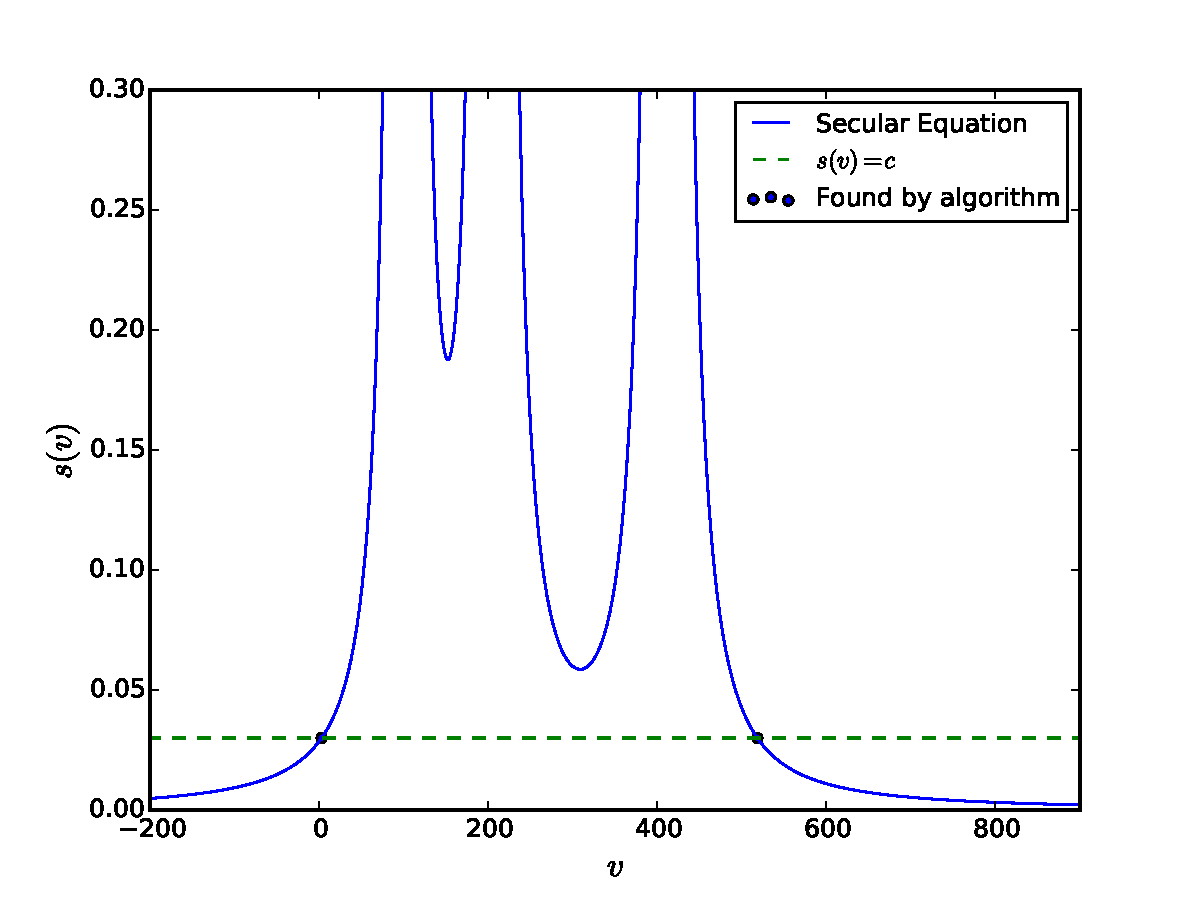
\includegraphics[width=0.9\linewidth]{../images/secular}
\caption{Plot of secular equation with three poles (all values made up to emphasize shape). Note that the function approaches infinity at the poles.}
\label{fig:secular}
\end{figure}


% The remainder of this paper expands and applies the ideas described
%previously. Implementation issues will be addressed, and a closer
%examination of the optimization problem's solution properties will be
%provided. The method will be illustrated using the IEEE RTS-96 test
%network. The paper will close with a discussion of how other
%components, such as voltage regulators, may affect the formulation.

%\section*{Acknowledgment}

%\section*{References}

% can use a bibliography generated by  as a .bbl file
% BibTeX documentation can be easily obtained at:
% http://www.ctan.org/tex-archive/biblio/bibtex/contrib/doc/
% The IEEEtran BibTeX style support page is at:
% http://www.michaelshell.org/tex/ieeetran/bibtex/
\bibliographystyle{IEEEtran}
% argument is your BibTeX string definitions and bibliography database(s)
%\bibliography{IEEEabrv,../bib/paper}
\bibliography{powerTechBib}
%
% <OR> manually copy in the resultant .bbl file
% set second argument of \begin to the number of references
% (used to reserve space for the reference number labels box)
%\begin{thebibliography}{16}


%\end{thebibliography}

\end{document}


